\documentclass[UTF8]{ctexart}
%\usepackage[margin=1.5cm]{geometry} %設定四個邊界皆為 1.5 cm
\usepackage[left=2cm, right=2cm, top=1.5cm, bottom=1.2cm]{geometry} %設定左邊界2cm,右邊界2cm,上邊界1.5cm, 下邊界 1.2cm
\setlength{\parindent}{0pt} %開頭不縮排

\usepackage{mathtools}

\usepackage{pgfplots}       % 使用pgfplots繪圖工具包
\pgfplotsset{width=7cm,compat=1.13} % 圖片繪制的寬度是7cm,使用的pgfplots版本是1.13

\usepackage{graphicx} %插入圖片函式庫
\usepackage{caption}
\usepackage{subfigure}

%\usepackage{comment} %多行註解函式庫

\begin{document}
\begin{CJK*}{UTF8}{song}
%\thispagestyle{empty} %首頁頁碼空白
\setlength{\baselineskip}{20pt} %全部行距皆為 30 points

%標題
\begin{center}
\begin{LARGE} 
\textbf{Debye-sears effect Experiment 結報} \\
\end{LARGE}
\begin{large} 
B5組 0412107 陳麒升、0412001 陳勁宇  
\end{large}
\end{center}

%%%%%%%%%%%%%%%<1頁%%%%%%%%%%%%%%%%%%
%動機
\begin{large}
\textbf{1.實驗動機與目的:} \\
\end{large}
利用Debye-sears effect分別在不同介質(本實驗使用水、鹽水(5\%)、酒精(95\%) )中的性質,以及於不同介質中的projection patterns of standing ultrasonic waves來計算介質中的聲音傳播速度。 \\
 \\
%
% 你認為或發現的實驗操作重點方式,條列式 ≤ 五項
\begin{large}
\textbf{2.實驗操作重點方式:} \\
\end{large}
◆於實驗操作方面我們組別認為需要注意的有: \\
(1) 注意線路品質、線路是否都能穩定收發訊號。 \\
(2) 注意架設超聲波波源之平台務必保持水平(可由水平儀驗證調整之)。 \\
(3) 注意待測溶液中盡量不要有小氣泡影響光路與聲音共振。 \\
(4) 雷射扣具與容器間須保持絕對乾燥。 \\
(5) 實驗時盡量不要動到放置實驗儀器之桌面,以防震動所造成之光斑判斷誤差。 \\

%
%%%%%%%%%%%%%%%%%%%%%%%%%%%%%%%%%%%%%%


%%%%%%%%%%%%%%%2~5頁%%%%%%%%%%%%%%%%%%
% 附課堂上操作的原始數據資料等
\begin{large}
\textbf{3.實驗raw data:} \\
\end{large} 
(1)實驗一 : \\
◆$H_{2}O$ : \\
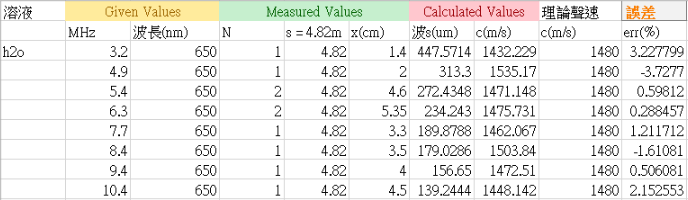
\includegraphics[width = 1.0\textwidth]{EXP1_H2O.png} \\

◆$NaCl (5\%)$ : \\
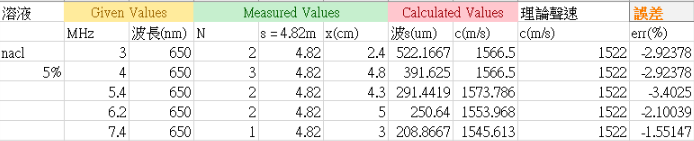
\includegraphics[width = 1.0\textwidth]{EXP1_NACL.png} \\

\newpage %強制分頁

◆$C_{2}H_{5}OH (95\%)$ : \\
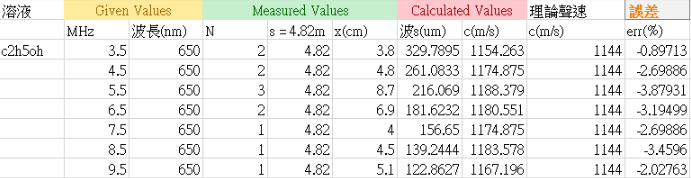
\includegraphics[width = 1.0\textwidth]{EXP1_C2H5OH.png} \\
\\

(2)實驗二(add lens) : \\
◆$H_{2}O$ : \\
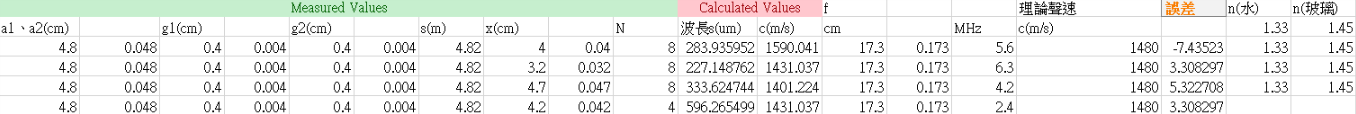
\includegraphics[width = 1.0\textwidth]{EXP2_LENS_H2O.png} \\

◆$NaCl (5\%)$: \\
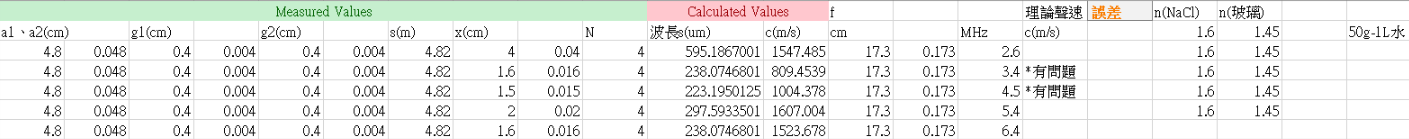
\includegraphics[width = 1.0\textwidth]{EXP2_LENS_NACL.png} \\

◆$C_{2}H_{5}OH (95\%)$ : \\
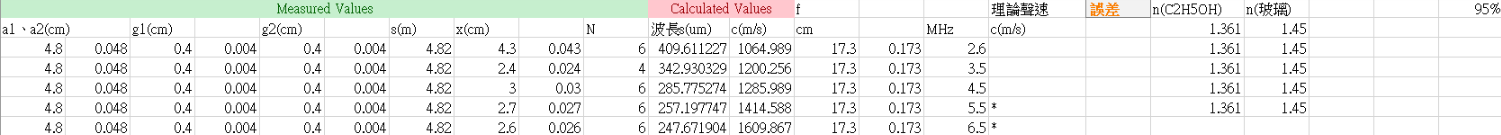
\includegraphics[width = 1.0\textwidth]{EXP2_LENS_C2H5OH.png} \\
\\

接下來之附件為附上方格紙的實驗光斑raw data紀錄結果。

\newpage



% 資料分析數據整理
\begin{large}
\textbf{4.資料分析數據整理: } \\
\end{large}
(1)實驗一 : 由3.部分之資料可知,三種介質在聲波源頻率為約$6.3MHz$左右時$x$會有一個極大值,並以此為中心向兩向頻率遞減。因此推斷此套實驗器材之紅光雷射在$6.3MHz$左右時振幅為最大值。此外,無論在何種介質中所得聲音速度的實驗誤差均不大($0\%$至$3\%$內)。 \\


(2)實驗二 : 由3.部分之資料可知,並以實驗一中所得$6.3MHz$左右時各介質聲音速度為參考基準,可以發現 : \\
1. $H_{2}O$ 方面 :  在聲波源頻率為$5.6MHz$時實驗所得聲速微過大,但尚在可接受範圍中($7\%$誤差)。 \\
2. $NaCl (5\%)$ 方面 : 在聲波源頻率為$3.4MHz$ 和 $4.5MHz$時實驗所得聲速過小($35\%$誤差)。\\
3. $C_{2}H_{5}OH (95\%)$ 方面 : 在聲波源頻率為$5.5MHz$ 和 $6.5MHz$時實驗所得聲速過大($43\%$誤差)。\\
 \\
%%%%%%%%%%%%%%%%%%%%%%%%%%%%%%%%%%%%%%%

%%%%%%%%%%%%%%1~2頁%%%%%%%%%%%%%%%%%%

% 分析結果,系統誤差來源,數據或方式上的討論 等等,結論 (含問題回答或思考)
\begin{large}
\textbf{5.分析結果與誤差來源討論 :} \\
\end{large}
(1) 於介質為水的實驗中可合理推論水中應有雜質影響實驗結果。 \\
(2) 於實驗二中所使用的透鏡表面有些括痕,使雷射產生成像誤差。 \\
(3) 手工描繪之光斑紀錄難免會有人為判斷誤差。 \\
 \\


% 如何改進(可有可無,若有請討論原因)
\begin{large}
\textbf{6.如何改進實驗: } \\
\end{large}
(1) 為了得到較完美之光學實驗結果,建議如果資源允許,能在暗房中配合氣墊光學桌及感光底片來進行實驗降低誤差。 \\
(2) 關於光斑圖案、$N$、$x$之實驗記錄與計算,如果資源允許,希望能於暗房中將屏幕換為感光CCD或potodiode陣列等感光電子元件,接收光電訊號配合程式自動運算獲得較精確(減少人為操作因素)之實驗結果並且可以節省人力。\\
(p.s.目前有想到之解決方案如下: (環境皆以氣墊光學桌+暗房為前提) \\
方案一: 將感光零件之類比訊號線接入$Arduino$/$ARM$等開發平台以韌體進行初步雜訊處理,並再利用$Python$界接資料流(這裡推薦將光電資料轉成$RS-485$協定透過Serial進開發板或電腦中)進行運算與繪圖,再將運算結果匯出成為csv檔案直接轉入$SQL$資料庫中儲存以方便大量分析與處理。\\
方案二: 利用Webcam或ip攝影機直接拍攝光學屏幕,將拍攝結果利用$OpenCV$或$LabVIEW$進行影像辨識(由於場景單純(黑底+紅光斑),因此這裡推薦以邊緣梯度辨識演算法實作。)) \\
 \\

\newpage

%列出猜考資料,各成員對此結報貢獻在何處
\begin{large}
\textbf{7.Reference: } \\
\end{large}
(1) e3上之實驗講義, "SOUND WAVE CONTROLLER SC600", 2018 \\
(2) gampt, "Debye-Sears effect",  http://www.gampt.de \\
 \\


\begin{large}
\textbf{8.組員貢獻分布: } \\
\end{large}
所有實驗與結報數據分析討論均是我們同組2人共同完成。 \\
(此次結報之~\LaTeX{} 格式繕打為 0412107 陳麒升負責 )

%$\sum_{i=1}^{n} f(x)$

\end{CJK*}
\end{document}